\section{Theory of Operations}
\subsection{Block Diagram}
\begin{figure}[h]
  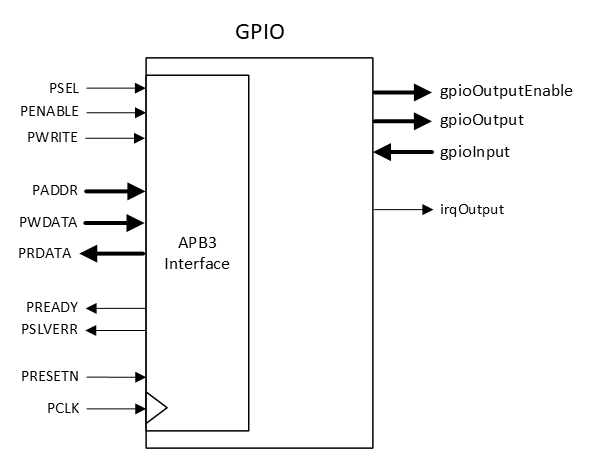
\includegraphics[width=0.80\textwidth]{images/uart-block-diagram.png}
  \caption{UART Block Diagram}\label{fig:block-diagram}
\end{figure}

\subsection{APB Interface}
The UART uses the APB interface for configuration and data transfer:
\begin{itemize}
  \item Configuration registers mapped to APB address space
  \item Separate TX/RX control registers
  \item Status registers for error reporting
  \item Double-buffered data registers
\end{itemize}

\subsection{Baud Rate Generation}
\begin{itemize}
  \item Programmable divisor: $\text{clocks\_per\_bit} = \frac{\text{clock\_freq}}{\text{baud\_rate}}$
  \item Automatic baud rate calculation
  \item Update synchronization to prevent glitches
\end{itemize}

\subsection{Data Framing}
\begin{itemize}
  \item Start bit detection
  \item Majority voting on sample points
  \item Optional parity generation/checking
  \item Configurable stop bits (fixed at 1 in current implementation)
\end{itemize}

\subsection{Error Handling}
\begin{itemize}
  \item Parity error detection
  \item Framing error detection
  \item Overrun detection
  \item Clearable error flags
\end{itemize}